\documentclass[14pt]{extarticle}
\usepackage{amsmath}
\usepackage{amssymb}
%\usepackage{tikz}
%\usetikzlibrary{calc}
%\usetikzlibrary{trees}
\usepackage{hyperref}
\usepackage{graphicx}
\graphicspath{ {../../chap09/} }
\usepackage[top=0.75in, bottom=0.75in, left=0.75in, right=0.75in]{geometry}
%\newcommand*{\Scale}[2][4]{\scalebox{#1}{\ensuremath{#2}}}%
\usepackage[shortlabels]{enumitem}
\usepackage[most]{tcolorbox}
\definecolor{bg}{RGB}{255,249,227}
% \usepackage{showframe}
\title{\vspace{-5ex}Math 208 Section 9.4}
\date{\vspace{-10ex}}
%\usepackage{multicol}
%\setlength{\columnsep}{1cm}
\setlength{\parindent}{0pt}
\usepackage{parskip}
\setlength{\parskip}{10pt} % 1ex plus 0.5ex minus 0.2ex}
%\usepackage{ragged2e}


\begin{document}
	\maketitle		
	\section*{Homework, Reading, and Other}
	\begin{itemize}
		\item Section 9.1
		\item Section 9.2
		\item Section 9.4
	\end{itemize}

	\section{Goals}
	\begin{itemize}
		\item Understand the meaning of \textit{instantaneous rate of change}.
		\item Use the four-step process to find a derivative.
		\item Find the equation of a tangent line.
	\end{itemize}
		
\section{Section 9.4: The Derivative}
\subsection{Introduction} The derivative gives us a mathematical method to determine rates of change. Consider driving in a car. What changes is your position. We are all familiar with the \textit{average rate of change}, i.e. miles per hour.

Say that, while driving, at 9am you passed mile marker 120 and then at 11am you passed mile marker 250. What is your average rate of change?

$$\frac{(250-120)\text{ miles}}{(11-9)\text{ hours}}= \frac{130 \text{ miles}}{2 \text{ hours}}= 65 \text{ miles per hour}$$

Certainly, you were not driving 65 miles per hour during the whole trip, sometimes faster and sometimes slower. This you determine from your speedometer and is the \textit{instantaneous rate of change}.

Mathematically, the average rate of change for a given function, $f(x)$ at $x=a$ to $x=a+h$ is:
$$\frac{f(a+h)-f(a)}{(a+h)-a} = \frac{f(a+h)-f(a)}{h} \text{ for }a\neq 0$$

Now let's consider the instantaneous rate of change.
\begin{tcolorbox}[enhanced jigsaw,colback=bg,boxrule=0pt,arc=0pt] 
	\textbf{Instantaneous rate of change} for a given function, $f(x)$ at $x=a$ is
	\begin{align*}
		\lim_{h\to 0}\frac{f(a+h)-f(a)}{h}
	\end{align*}
	if the limit exists.
\end{tcolorbox}

\subsection{Secant and Tangent Lines}
A line connecting and through any two points, $a$ and $a+h$, on the graph of a function is called a \textit{secant line}. The slope of this line is the average rate of change between $a$ and $a+h$.
$$\frac{f(a+h)-f(a)}{h} \text{ for }a\neq 0$$

\begin{center}
	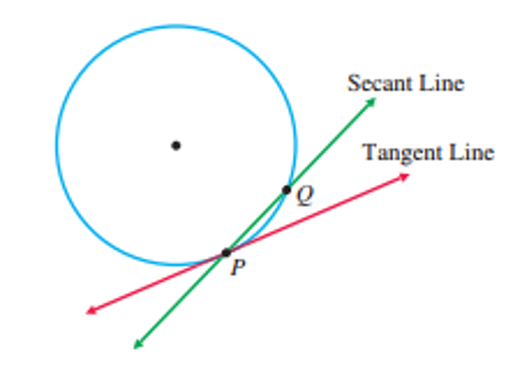
\includegraphics[width=0.5\textwidth]{9-4-20a}
\end{center}
A line that intersects a circle in exactly one point is called a \textit{tangent line}. For a function, we would say that the tangent line at a given point is the straight line that "just touches" the curve at that point. Leibniz defined it as the line through a pair of infinitely close points on the curve.

The slope of the tangent line is the instantaneous rate of change at the point $x=a$.
$$\lim_{h\to 0}\frac{f(a+h)-f(a)}{h}$$

\subsubsection*{Some Graphs}
\begin{itemize}
	\item Secant line to tangent line, \url{https://www.desmos.com/calculator/faudtsxdzy}
	\item Distance-velocity-accelerate, \url{https://www.desmos.com/calculator/jgxmedmm8n}
\end{itemize}

\subsection*{The Derivative}
\begin{center}
	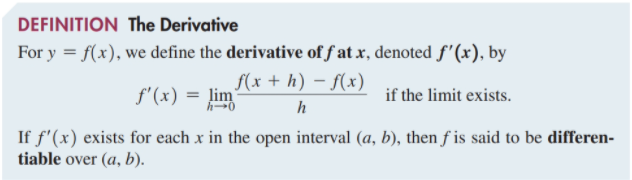
\includegraphics[width=0.9\linewidth]{9-4-1}
\end{center}
Not every function has a derivative at every point, $x=a$, but if the derivative exists, we indicate it by $\mathbf{f'(x)}$.

\begin{center}
	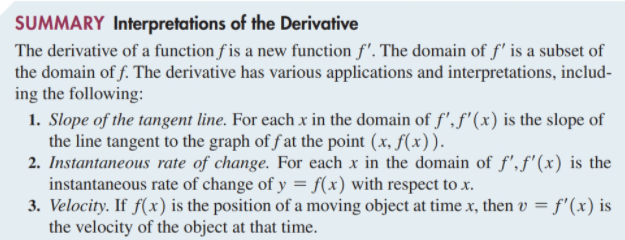
\includegraphics[width=0.9\linewidth]{9-4-2}
\end{center}
Often, you may be asked to find the equation of the tangent line. Recall that the equation of a line may be given in point-slope form:
$$(y-y_o) = m(x-x_0)$$
or in slope-intercept form:
$$y=mx+b$$
Since $f'(a) = m$ at $x=a$, it is best to \textbf{use point-slope form}. Then:
\begin{align*}
	x_0 &= a \\
	y_0 &= f(a) \\
	m & = f'(a)
\end{align*}

\subsection{The Four-step Process}
Follow this four step process to find the derivative of any function for which the derivative exists.
\begin{center}
	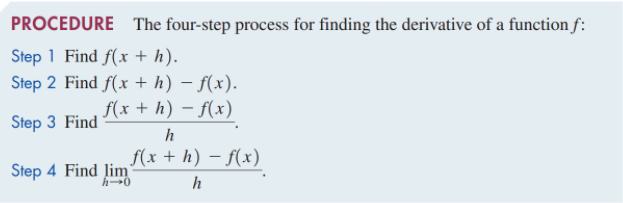
\includegraphics[width=0.9\linewidth]{9-4-3}
\end{center}

\subsubsection{Examples}
Find the derivative at $x$ of $f(x) = -16x^2 +80x+6$

\textbf{Step 1:} $f(x+h)$
\begin{align*}
	f(x+h) & = -16(x+h)^2 + 80(x+h) + 6 \\
	&= -16(x^2 + 2xh+h^2) + 80x + 80h + 6 \\
	&= -16x^2 -32xh -16h^2 + 80x + 80h + 6 
\end{align*}

\textbf{Step 2:} $f(x+h) - f(x)$
\begin{align*}
	f(x+h)-f(x) &= -16x^2 -32xh -16h^2 + 80x + 80h + 6 - (-16x^2 +80x+6) \\
	&= -16x^2 -32xh -16h^2 + 80x + 80h + 6 +16x^2 -80x -6 \\
	&= -32xh -16h^2 +80h
\end{align*}

\textbf{Step 3:} $\frac{f(x+h) - f(x)}{h}$
\begin{align*}
	\frac{f(x+h) - f(x)}{h} &= \frac{-32xh -16h^2 +80h}{h} \\
	&= -32x -16h +80
\end{align*}

\textbf{Step 4:} $\lim_{h\to 0}\frac{f(x+h) - f(x)}{h}$
\begin{align*}
	\lim_{h\to 0}\frac{f(x+h) - f(x)}{h} &= \lim_{h\to 0}(-32x -16h +80) \\
	&= -32x  +80
\end{align*}



\noindent\rule{\textwidth}{1pt}
{\footnotesize Copyright (C) 2021 Garold Dalton --- Released under GNU General Public License v3.0}


\cleardoublepage


\end{document}
